\section{Main Result}
    This section describes the specific steps taken and the overall development process of the project. It is split into several sections where arguments for major decisions are presented and challenges encountered are examined as well.
    
    The \nameref{techstack} subsection presents specific technologies used, such as programming language of choice and different development libraries. It also lists computer specifications that were used to perform all of the code running tasks and explains potential limitations.
    
    The second subsection, \nameref{twitterdata}, discusses how twitter data was gathered, how it was preprocessed and why it had to be done, while also explaining challenges associated with it.
    
    In \nameref{devlstm} subsection, the whole development process of \gls{lstm} is described, covering everything from development decisions, training, validation and testing of the neural network. Evaluation and discussion of obtained results is described in \nameref{evalstm} by comparing them with existing similar work performed previously. 
    
    The \nameref{graphnetwork}

    \subsection{Technology Stack} \label{techstack}
        The chosen technology stack is as follows:
        \begin{itemize}
            \item Programming language Python version 3.7. There is a reason why Python is the de facto language for all purposes Machine Learning, Deep Learning, Data Science and Analysis, and this is because of the vast amount of libraries that enable the developer to easily incorporate the functionality in any project. Nonetheless, the core calculations of those libraries are done in C/C++ language and Python is used as a wrapper for easy access and compatibility, which makes memory intensive computations all the more efficient.
            
            \item The most popular library that delivers upon the objectives of the project is TensorFlow, and as such it is used in this project. It's popularity speaks volumes as there is a vast amount of guides easily accessible and extendable into solving complex problems (such as Recognizing Textual Entailment, for example). Also, the documentation is full with up to date details, examples and clearly explaining differences between versions, whether past or upcoming changes.
            
            \item Tweepy was chosen to be used as Twitter API access library, because, first of all, is one of the not many libraries that are still maintained and updated today, constantly providing more and more flexibility with gathering of Twitter Data, and secondly, because of documentation providing lots of examples how to quickly set up and get up to speed.
            
            \item Anaconda was used as a package and dependency manager for Python, allowing easy and quick addition of various external libraries (Tweepy, TensorFlow and various sub dependencies). Moreover, PyCharm was used to fulfil the role of Integrated Development Environment for Python, mostly because of it having a lot more features than the free counterparts, as students can get Ultimate license free of charge for a year.
            
            \item Computer specifications include 16.0 GB of \gls{ram}, which was a limitation at some points during the \gls{snli} corpus (details about it are explained later) data processing (calculating data features list and classification scores). For \gls{lstm} training, evaluation and overall running, GeForce GTX 1080 Ti was used with 11.0 GB of dedicated memory and 8.0 GB of shared memory, making use of multiprocessing capabilities of the graphics card. All other calculations were performed on Intel i7-7700k @ 4.20 GHz speed.
        \end{itemize}

    \subsection{Mining of Twitter Data} \label{twitterdata}
        Currently, the implementation of Data Mining comprises of the following steps:
        \begin{itemize}
            \item As the program connects to Twitter API, it fetches a single tweet based on specified parameters (topic or hashtag, amount to fetch, etc.).
            
            \item The fetched tweet is preprocessed, by removing stop words and performing lemmatization.
            
            \item Afterwards, the resulting text is saved into \gls{csv} file format, along with meta data about the tweet (timestamp, like count, etc.) for later use (such as passing it through \gls{lstm} predictions).
        \end{itemize}
        
        The importance to perform an intermediate saving of the data into \gls{csv} file is to alleviate the pressure on \gls{ram}, there is no need to hold all the data in memory at this point.
        
    \subsection{Development of Long Short-Term Memory Network} \label{devlstm}
        The \gls{lstm} was developed utilising the \gls{snli} corpus, which contains 570,152 sentence pairs labelled \textit{entailment}, \textit{neutral}, \textit{contradiction} or \textit{-} \autocite{Bowman2015ALA}. The \textit{-} pairs were removed from the data set as they indicate a lack of consensus from the annotators. Next, these pairs are split into three separate data sets. The training set consists of 549,367 sentence pairs, while validation and testing sets contain 9,842 and 9,824 respectively. The argument for using \gls{snli} data sets is that the sheer size of it make it feasible to train a neural network.
        
        Next, instead of word2vec, the word embeddings trained from \gls{glove} are used \autocite{Pennington2014GloveGV}. This is because \gls{glove} covers more words in the \gls{snli} data set than word2vec. More precisely, while \gls{snli} contains 37K unique tokens, around 4.1K of them cannot be found in \gls{glove}, while 12.1K in word2vec.
        
        For training, Adam method is used with hyperparameters $\beta_1$ = 0.9 and $\beta_2$ = 0.999 for optimisation \autocite{Kingma2015AdamAM}. Initial learning rate is set to 0.001 and weight decay equals to 0.95. A three-class classification is performed (entailment, neutral, contradiction). Accuracy is used as an evaluation metric.
        
        \textit{Batch size, dimension of hidden states and output vector size parameters will be discussed in July's progress report.}
        
        The \gls{lstm} itself is bidirectional. This means that the input is processed in two directions - words used at the beginning of the sentence are used to understand the following words after that, and words that come at the end of the sentence are used to predict what the beginning of the sentence should look like. The advantage of using bidirectional \gls{lstm}s is that they replicate the way humans process sentences and meanings. When reading a sentence, previously read words are required to understand what is being said next, and vice versa.
        
        To combat overfitting, L2 Regularization is used to minimize losses and input keep probability is set to 10\%. This means that 10\% of the input is randomly chosen to be remembered that lead to the output, while the rest is discarded. Accuracy is calculated by looking at a number of correct classifications versus actual classifications.
        
    \subsection{Evaluation and Comparison of LSTM Performance} \label{evalstm}
        \textit{Due for July's progress report as still constantly testing different parameters and their combinations.}
    
    \subsection{Graph Network Construction} \label{graphnetwork}
        \textit{Due for July's progress report.}
    
    \subsection{Bipolar Argumentation Framework Analysis} \label{bapanalysis}
        \textit{Due for July's progress report or early August.}
    
% The chapter reports the contribution of your work.  For example, it could contain the following sub-sections to summarise the contribution of the project: Theoretical Development, Analysis and Design, Implementation and Experimental Work, Results, Observation and Discussion.

% \subsection{Maths}
% \begin{equation}\label{eq:BS}
% \frac{\D S_t}{S_t} = r \D t + \sigma \D W_t,
% \qquad S_0>0,
% \end{equation}

% The equation $\sigma = m a$ follows easily~\citep{phdthesis}.

% \subsection{Glossary and acronyms}

% \Glspl{Linux} and other Unix operating systems are better then Windows because they support \gls{lvm} out of the box~\citep{Joh11}\insertref{reference missing}. 

% \subsection{Figures}
% Here is an example of how to insert a picture:

% \begin{figure}[!ht]
% \centering
% \subfigure{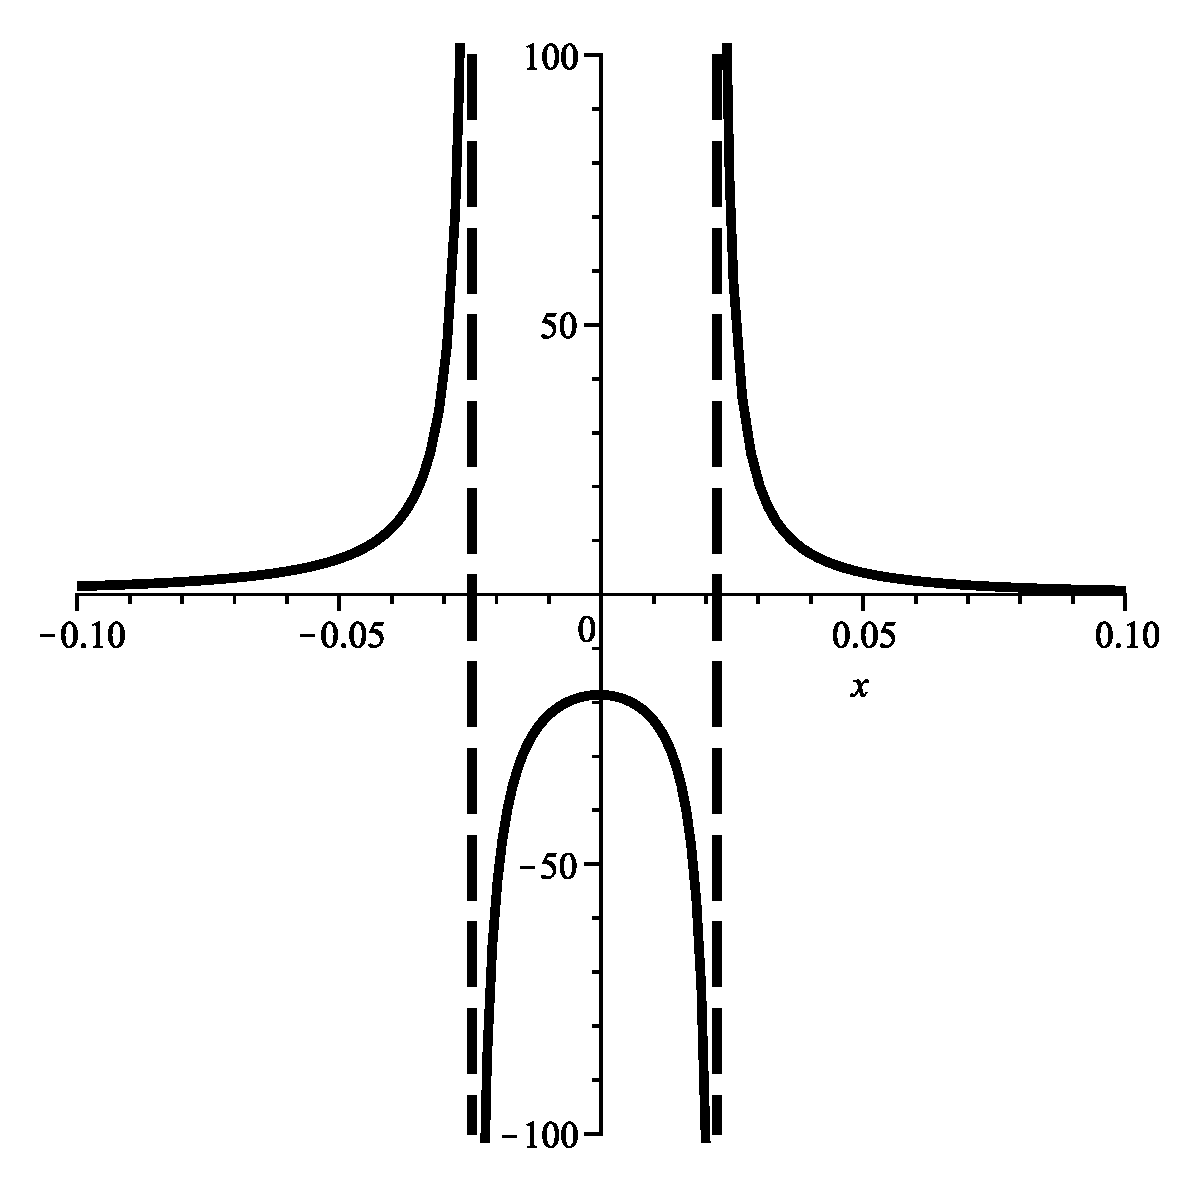
\includegraphics[scale=0.2]{figures/Picture.eps}}
% \caption{This is the caption for the figure.}
% \label{fig:Pict}
% \end{figure}


% \begin{figure}[!ht]
% \centering
% \missingfigure{If you know there will be a figure, but you still need to create it.}
% \caption{This is the caption for the figure which is not even present.}
% \label{fig:PictMis}
% \end{figure}

% \todo{This is a small Todo, please take care!}

% or two side-by-side pictures:

% \begin{figure}[!ht]
% \centering
% \subfigure{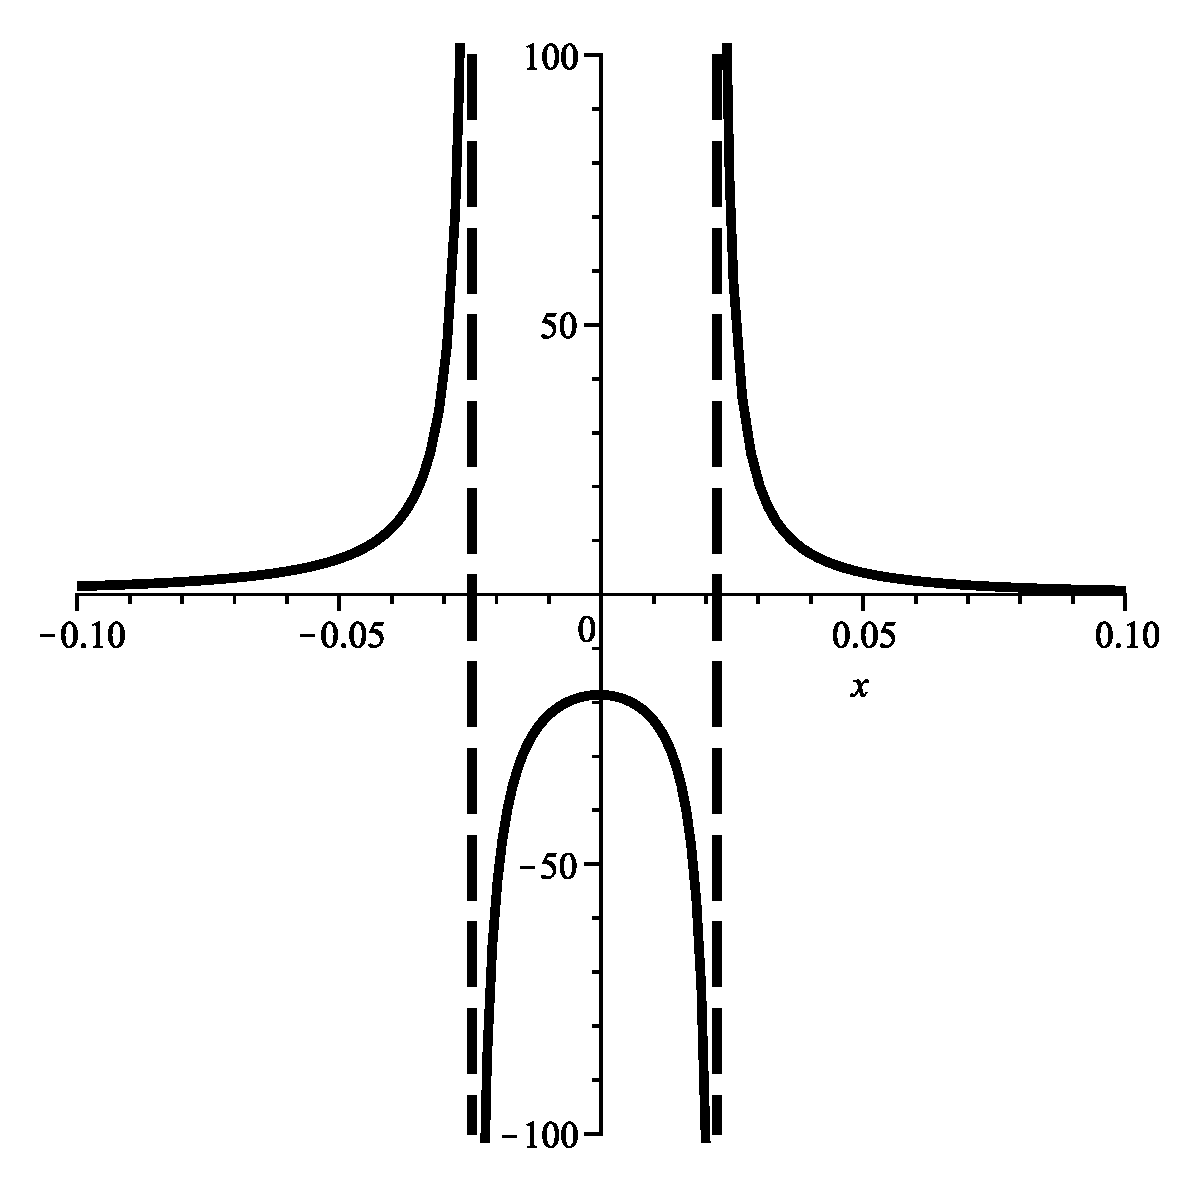
\includegraphics[scale=0.3]{figures/Picture.eps}}
% \hspace{15pt}
% \subfigure{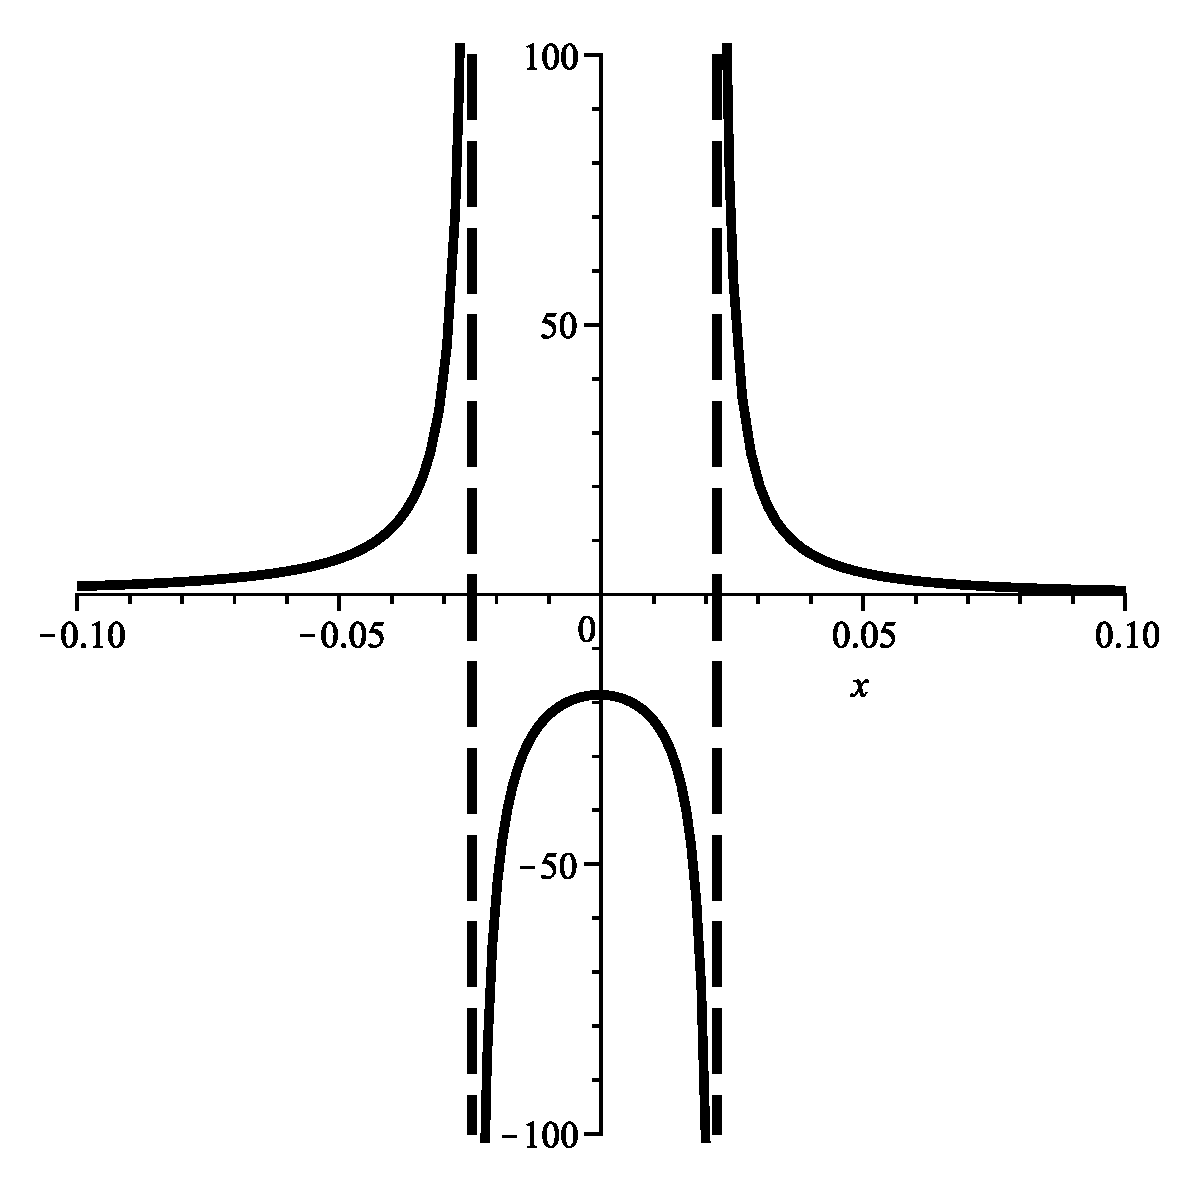
\includegraphics[scale=0.3]{figures/Picture.eps}}

% \caption{Another caption}
% \label{fig:Pict2}
% \end{figure}



% \subsection{Table}
% Lorem ipsum dolor sit amet, consetetur sadipscing elitr, sed diam nonumy eirmod tempor invidunt ut labore et dolore magna aliquyam erat, sed diam voluptua. At vero eos et accusam et justo duo dolores et ea rebum. Stet clita kasd gubergren, no sea takimata sanctus est Lorem ipsum dolor sit amet. Lorem ipsum dolor sit amet, consetetur sadipscing elitr, sed diam nonumy eirmod tempor invidunt ut labore et dolore magna aliquyam erat, sed diam voluptua. At vero eos et accusam et justo duo dolores et ea rebum. Stet clita kasd gubergren, no sea takimata sanctus est Lorem ipsum dolor sit amet\explainindetail{This needs further explanation}.
% \begin{table}[!ht]
% 	\centering
% 	\begin{tabular}{|l|rl|}
% 		\hline
% 		Something & Someother & Thing \\
%   		Seems & to be & good\\
%   		\hline
%   	\end{tabular}
%   	\caption{Random data for a table.}
% \end{table}

% Lorem ipsum dolor sit amet, consetetur sadipscing elitr, sed diam nonumy eirmod tempor invidunt ut labore et dolore magna aliquyam erat, sed diam voluptua. At vero eos et accusam et justo duo dolores et ea rebum. Stet clita kasd gubergren, no sea takimata sanctus est Lorem ipsum dolor sit amet. Lorem ipsum dolor sit amet, consetetur sadipscing elitr, sed diam nonumy eirmod tempor invidunt ut labore et dolore magna aliquyam erat, sed diam voluptua. At vero eos et accusam et justo duo dolores et ea rebum. Stet clita kasd gubergren, no sea takimata sanctus est Lorem ipsum dolor sit amet.


% \section{Model calibration}
% \subsection{What is calibration?}
% Here is an example of a matrix\citep{website:fermentas-lambda} in $A\in\mathcal{M}_n(\RR)$:
% $$
% A = 
% \begin{pmatrix}
% a_{11} & a_{12} & \ldots & a_{1n}\\
% a_{21} & \ddots & \ddots  & \vdots\\
% \vdots &  \ddots & \ddots  & \vdots\\
% a_{n1} &  \ldots &  \ldots & a_{1n}.
% \end{pmatrix}
% $$

% \subsection{Numerical methods for calibration}
...


